% Dataset stats: HMDs-IAI
\begin{figure}[ht]
%\captionsetup[subfigure]{labelformat=empty}
\centering
\subfloat[\Gls{teental}]{\label{fig:dstats:HMDs:IAI:teen}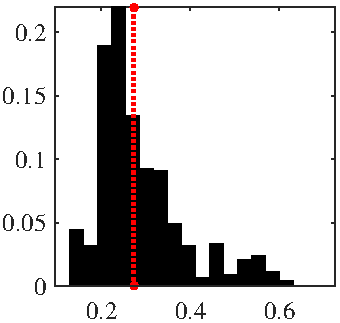
\includegraphics[scale=1]{dstats/HMDs-teen-IAI.pdf}} \hspace{0.5cm} 
\subfloat[\Gls{ektal}]{\label{fig:dstats:HMDs:IAI:ek}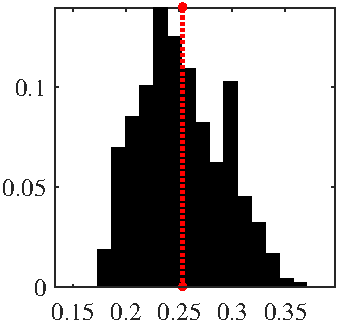
\includegraphics[scale=1]{dstats/HMDs-ek-IAI.pdf}} \\ 
\subfloat[\Gls{jhaptal}]{\label{fig:dstats:HMDs:IAI:jhap}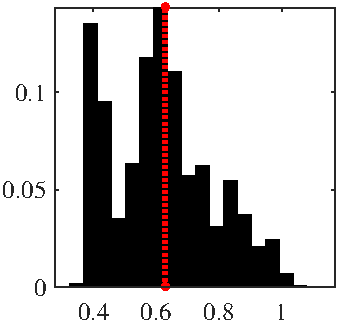
\includegraphics[scale=1]{dstats/HMDs-jhap-IAI.pdf}} \hspace{0.5cm} 
\subfloat[\Gls{rupak}]{\label{fig:dstats:HMDs:IAI:rupak}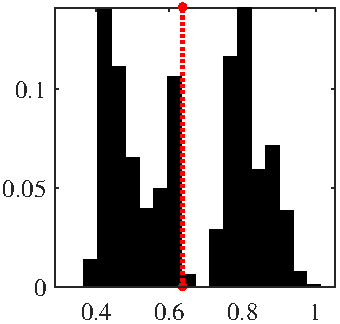
\includegraphics[scale=1]{dstats/HMDs-rupak-IAI.pdf}} \\ 
\caption[HMDs-IAI]{HMDs-IAI}\label{fig:dstats:HMDs:IAI}
\end{figure}
%
%
% Dataset stats: HMDs-IAInorm
\begin{figure}[ht]
%\captionsetup[subfigure]{labelformat=empty}
\centering
\subfloat[\Gls{teental}]{\label{fig:dstats:HMDs:IAInorm:teen}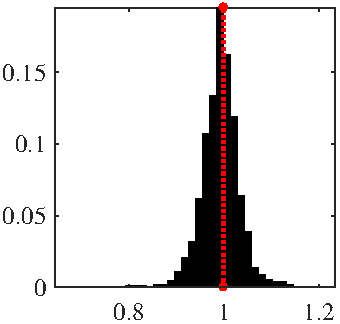
\includegraphics[scale=1]{dstats/HMDs-teen-IAInorm.pdf}} \hspace{0.5cm} 
\subfloat[\Gls{ektal}]{\label{fig:dstats:HMDs:IAInorm:ek}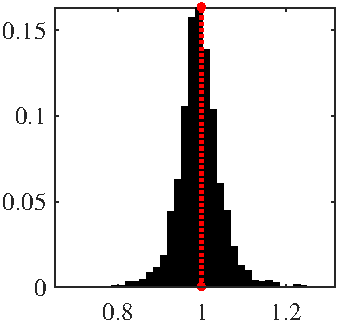
\includegraphics[scale=1]{dstats/HMDs-ek-IAInorm.pdf}} \\ 
\subfloat[\Gls{jhaptal}]{\label{fig:dstats:HMDs:IAInorm:jhap}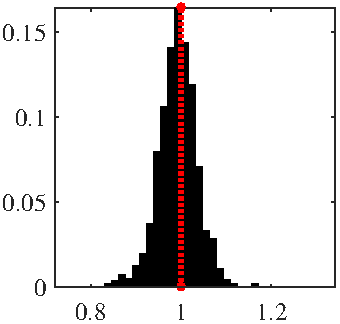
\includegraphics[scale=1]{dstats/HMDs-jhap-IAInorm.pdf}} \hspace{0.5cm} 
\subfloat[\Gls{rupak}]{\label{fig:dstats:HMDs:IAInorm:rupak}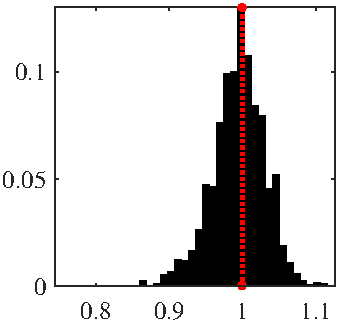
\includegraphics[scale=1]{dstats/HMDs-rupak-IAInorm.pdf}} \\ 
\caption[HMDs-IAInorm]{HMDs-IAInorm}\label{fig:dstats:HMDs:IAInorm}
\end{figure}
%
%
% Dataset stats: HMDs-ISI
\begin{figure}[ht]
%\captionsetup[subfigure]{labelformat=empty}
\centering
\subfloat[\Gls{teental}]{\label{fig:dstats:HMDs:ISI:teen}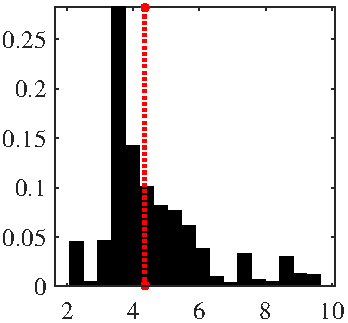
\includegraphics[scale=1]{dstats/HMDs-teen-ISI.pdf}} \hspace{0.5cm} 
\subfloat[\Gls{ektal}]{\label{fig:dstats:HMDs:ISI:ek}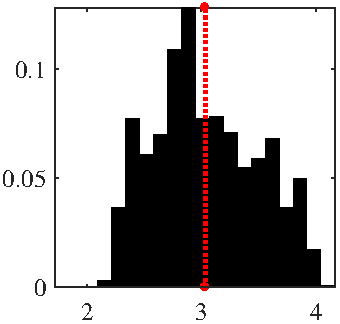
\includegraphics[scale=1]{dstats/HMDs-ek-ISI.pdf}} \\ 
\subfloat[\Gls{jhaptal}]{\label{fig:dstats:HMDs:ISI:jhap}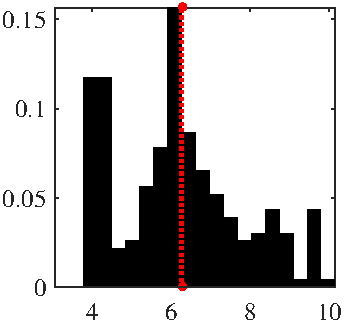
\includegraphics[scale=1]{dstats/HMDs-jhap-ISI.pdf}} \hspace{0.5cm} 
\subfloat[\Gls{rupak}]{\label{fig:dstats:HMDs:ISI:rupak}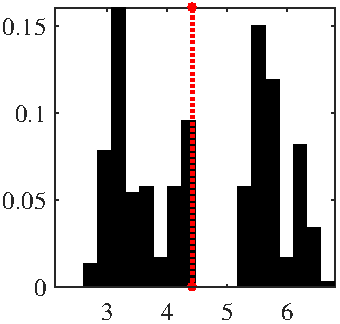
\includegraphics[scale=1]{dstats/HMDs-rupak-ISI.pdf}} \\ 
\caption[HMDs-ISI]{HMDs-ISI}\label{fig:dstats:HMDs:ISI}
\end{figure}
%
%
% Dataset stats: HMDs-ISInorm
\begin{figure}[ht]
%\captionsetup[subfigure]{labelformat=empty}
\centering
\subfloat[\Gls{teental}]{\label{fig:dstats:HMDs:ISInorm:teen}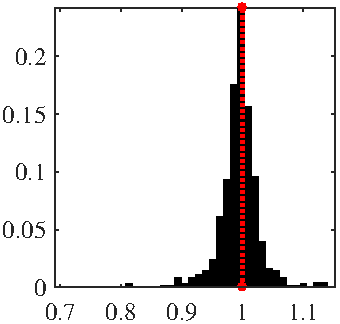
\includegraphics[scale=1]{dstats/HMDs-teen-ISInorm.pdf}} \hspace{0.5cm} 
\subfloat[\Gls{ektal}]{\label{fig:dstats:HMDs:ISInorm:ek}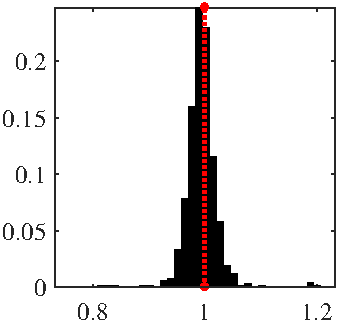
\includegraphics[scale=1]{dstats/HMDs-ek-ISInorm.pdf}} \\ 
\subfloat[\Gls{jhaptal}]{\label{fig:dstats:HMDs:ISInorm:jhap}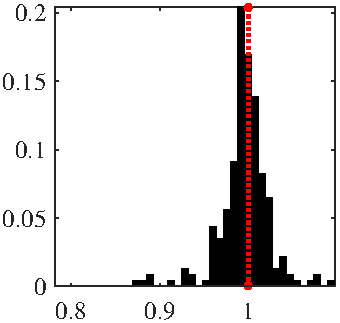
\includegraphics[scale=1]{dstats/HMDs-jhap-ISInorm.pdf}} \hspace{0.5cm} 
\subfloat[\Gls{rupak}]{\label{fig:dstats:HMDs:ISInorm:rupak}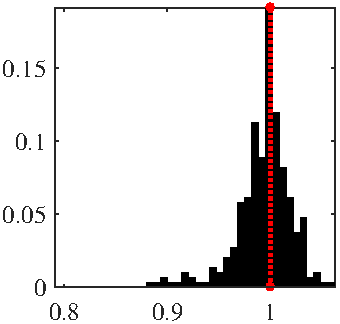
\includegraphics[scale=1]{dstats/HMDs-rupak-ISInorm.pdf}} \\ 
\caption[HMDs-ISInorm]{HMDs-ISInorm}\label{fig:dstats:HMDs:ISInorm}
\end{figure}
%
%